\section{Operationsleitung/OPL (Headquarter/HQ)}
\begin{figure}[htbp]
	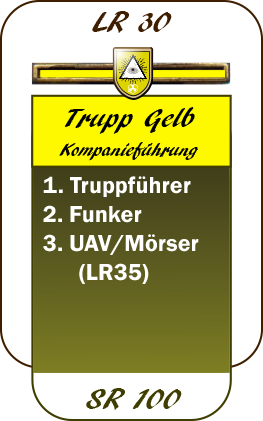
\includegraphics[width=50mm]{./img/truppenordnung/opl/opl.png}
	\caption{Beispiel einer OPL}
\end{figure}
Die OPL ist die höchste Instanz innerhalb einer Mission. Sie hat den Oberbefehl über alle Einheiten inne, koordiniert das allgemeine Vorgehen innerhalb der Mission und verwaltet die Zuordnung der unterstützenden Einheiten zu den kämpfenden Einheiten.Sie kommuniziert grundsätzlich nur über die Long-Range mit ihren untergeordneten Einheiten.\\
Die OPL ist folgendermaßen aufgebaut:
\begin{itemize}
	\item Operationsleiter/OPL (Commanding Officer(CO)): Der Oberbefehlshaber der Mission. Er gibt die Befehle und erstellt "den großen Plan".
	\item stellv. OPL (Executive Officer/XO): Unterstützt den OPL bei seinen Aufgaben, typischerweise beim Funken mit den untergeordneten Trupps. Kann jedoch auch alle weiteren Aufgaben übernehmen, die ihm der OPL überträgt - er ist Mädchen für alles. Bewährt hat sich das Prinzip, dass der OPL den eingehenden Funk übernimmt (Anfragen von anderen Trupps) und der stellv. OPL den ausgehenden Funk (Abfragen von Statusberichten, Übermittlung von neuen Befehlen).
\end{itemize}
Ergänzt werden kann die OPL durch maximal 4 Spieler, welche folgende Rollen einnehmen können:
\begin{itemize}
	\item Funker (Radio Operator/RO): ein zusätzlicher Funker, um die OPL zu unterstützen, kann auf eine Spezialrolle beschränkt sein und für diese eine eigene LR-Frequenz bekommen (so kann es z.B. bei einer Mission mit vielen Lufteinheiten sinnvoll sein, jemanden zu haben, der sich auf einer eigenen Frequenz nur um die Koordination der Lufteinheiten um das Flugfeld kümmert und zentraler Ansprechpartner aller Lufteinheiten für Start-/Landemanöver ist)
	\item Aufklärungsoffizier (Intelligence Officer/IO): Sammelt alle verfügbaren, relevanten Daten und leitet diese gegebenenfalls an andere Trupps weiter. Hat meistens eine eigene, "große" Drohne (Greyhawk/Global Hawk) zur Feindaufklärung.
	\item freie Rolle (maximal einmal): je nach Mission kann es sinnvoll sein, dem OPL einen Sanitäter, einen Nahsicherer, einen Fahrer o.Ä. zur Seite zu stellen
\end{itemize}
Je nach Größe und Struktur der Mission kann die OPL identisch sein mit
\begin{itemize}
	\item der Sektionsführung, falls nicht mehr als eine Sektion in der Mission existiert
	\item der Zugführung, falls die Mission nur aus einem Zug besteht (egal ob Infanteriezug, Panzerzug oder mechanisierte Infanterie). Dies ist die einzige Ausnahme, in der die OPL per Short-Range statt Long-Range mit ihren untergeordneten Einheiten kommuniziert.
\end{itemize}